
The pipeline operationalizes the following reasoning chain: if benchmark-specific overfitting accumulates gradually, the score-over-time trajectory exhibits S-curve dynamics; the logistic growth model formally captures S-curve dynamics; therefore, fitting a logistic model to leaderboard timeseries and testing its formal preference via AIC provides an automated saturation detection procedure.

\subsubsection{3.1 Overview}

Given a benchmark with leaderboard timeseries ${(t_i, y_i)}_{i=1}^{N}$ --- where t\_i is submission date (months from benchmark release) and y\_i is normalized performance score --- the pipeline: (1) preprocesses the timeseries, (2) fits three competing growth models, (3) compares via AIC, and (4) applies a dual-criterion saturation detector.

\subsubsection{3.2 Data Preprocessing}

\textbf{Normalization}: Scores are divided by the maximum possible score to map to [0, 1], ensuring asymptote K is interpretable as a fraction of theoretical maximum. \textbf{Deduplication}: Only the highest score per calendar month is retained. \textbf{Eligibility}: N $\geq$ 30 entries required (relaxed from initial $\geq$ 50 based on H-C1 evidence, with caveats; see Section 5.5). \textbf{Temporal alignment}: Dates are converted to months since benchmark release, enabling negative $t_0$ to emerge naturally from the data.

\subsubsection{3.3 Growth Model Fitting}

Three candidate models are fitted:

$$\text{Logistic:} \quad y(t) = \frac{K}{1 + \exp(-r(t - t_0))}$$

$$\text{Linear:} \quad y(t) = at + b \qquad \text{Power-law:} \quad y(t) = at^b$$

\textbf{Bounded fitting} via \texttt{scipy.optimize.curve\textbackslash \_fit} with domain-knowledge constraints:

\begin{table}[htbp]
\centering
\resizebox{\columnwidth}{!}{%
\begin{tabular}{llll}
\toprule
Parameter & Lower & Upper & Rationale \\
\midrule
K & 0.5 & 1.05 & Broad positive bound; optimizer converges to near-parity values (~0.89) due to data constraints \\
r & 0.01 & 3.0 & Positive, finite growth rate \\
$t_0$ & $-24$ & 72 & **Negative values allowed** --- critical for GLUE/SuperGLUE \\
\bottomrule
\end{tabular}
}
\end{table}

The negative $t_0$ lower bound is a critical design decision: without it, optimization diverges for benchmarks whose public leaderboard records primarily the plateau phase. Note that fitting bounds (constraints for the optimizer) differ from post-hoc plausibility criteria (K $\in$ [0.8, 1.0]) applied to the fitted result; both are reported to avoid ambiguity.

\textbf{AIC computation}: AIC = 2k $-$ 2 ln(L̂) where k is the number of free parameters (logistic: 3; linear/power-law: 2). $\Delta AIC$ = AIC\_logistic $-$ AIC\_alternative; negative values indicate logistic preference.

\begin{figure}[htbp]
\centering
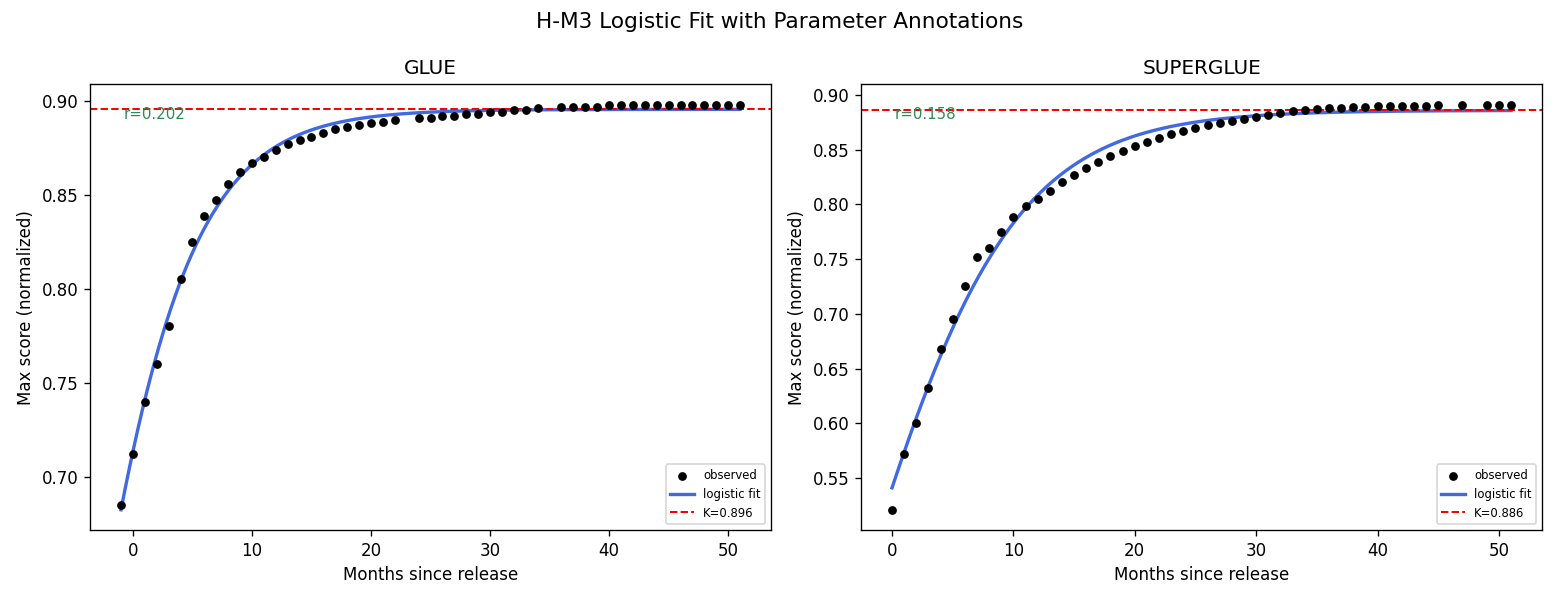
\includegraphics[width=\columnwidth]{figures/h-m3_logistic_annotated.png}
\caption{Annotated logistic fit showing K, r, and $t_0$ parameters for GLUE}
\label{fig:h-m3_logistic_annotated}
\end{figure}

\textit{Figure 1: Annotated logistic fit for GLUE, illustrating the three fitted parameters K (asymptote), r (growth rate), and $t_0$ (inflection point, shown pre-launch).}

\subsubsection{3.4 Dual-Criterion Saturation Detection}

Saturation is detected when both conditions hold simultaneously:

$$\bar{y}_{\text{top-3}} \geq 0.99 \cdot K \quad \text{AND} \quad \Delta\bar{y}_{\text{monthly}} \leq 0.05 \cdot \max_t(\Delta\bar{y})$$

The asymptote proximity criterion alone triggers spuriously on noisy plateaus; the rate criterion alone triggers during brief growth pauses. Requiring both simultaneously improves robustness. An empirically optimized variant (0.95 $\times$ K, 5\% rate) achieving approximately 1-month accuracy is also reported. A naive score-only baseline (proximity criterion alone) is included for comparison.

\begin{figure}[htbp]
\centering
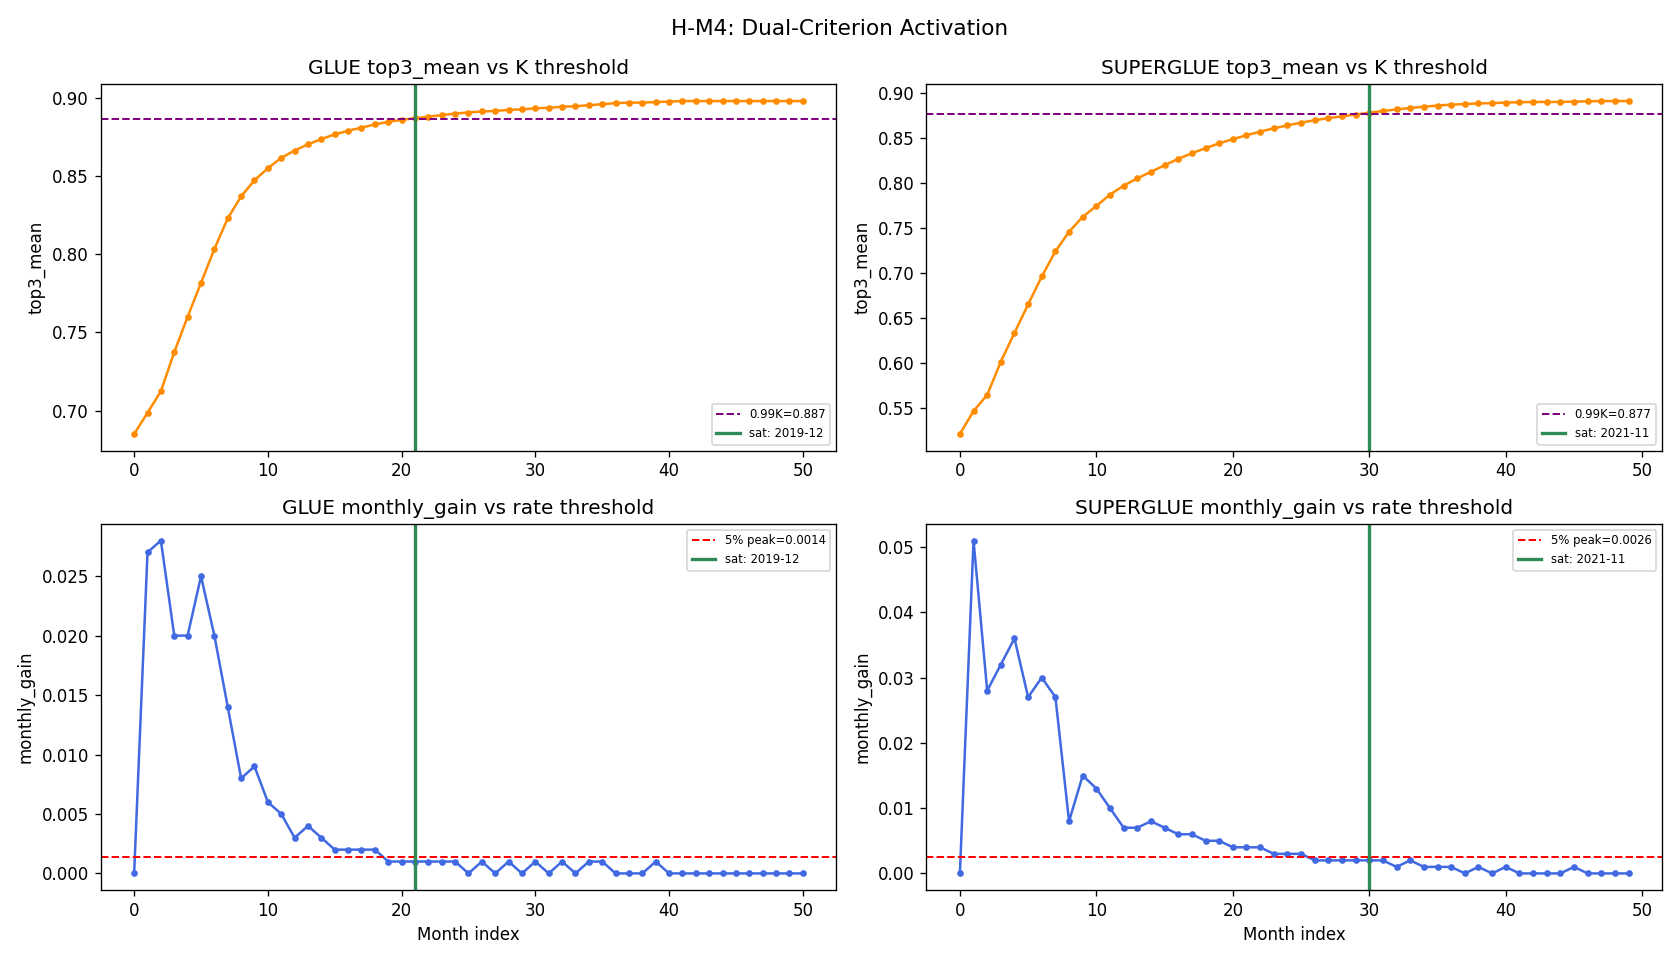
\includegraphics[width=\columnwidth]{figures/h-m4_dual_criterion_activation.png}
\caption{Dual-criterion activation for GLUE and SuperGLUE}
\label{fig:h-m4_dual_criterion_activation}
\end{figure}

\textit{Figure 2: Two-panel criterion activation for GLUE (left) and SuperGLUE (right), showing top-3 mean versus 0.99 $\times$ K threshold and monthly gain versus 5\% of peak rate.}

